\section{Massfits for signal and normalization channel}
\label{sec: fitting}

This section describes the nominal fits to the invariant mass distribution of $\Bs\to\Ds\kaon\pion\pion$ and $\Bs\to\Ds\pion\pion\pion$ candidates after all selection steps, described in the previous Sections, are applied. 
The obtained yields are summarized in Tab. \ref{tab: SigYields}.

\subsection{Fit to $\Bs\to\Ds\pion\pion\pion$ candidates}
\label{subsec: NormFit}

An unbinned maximum likelihood fit is performed to the invariant mass distribution of $\Bs\to\Ds\pion\pion\pion$ candidates. 
As discussed in Sec. \ref{subsec: signalmodel}, the fit is given as the sum of the double gaussian signal model, the sum of three bifurcated gaussians to model the partially reconstructed $\Bs\to\Ds^{*}\pion\pion\pion$ background, as well as an exponential to account for combinatorial background. The invariant mass distribution and the fit to it is shown in Fig. \ref{fig: BsDs3piFit}.

\begin{figure}[h]
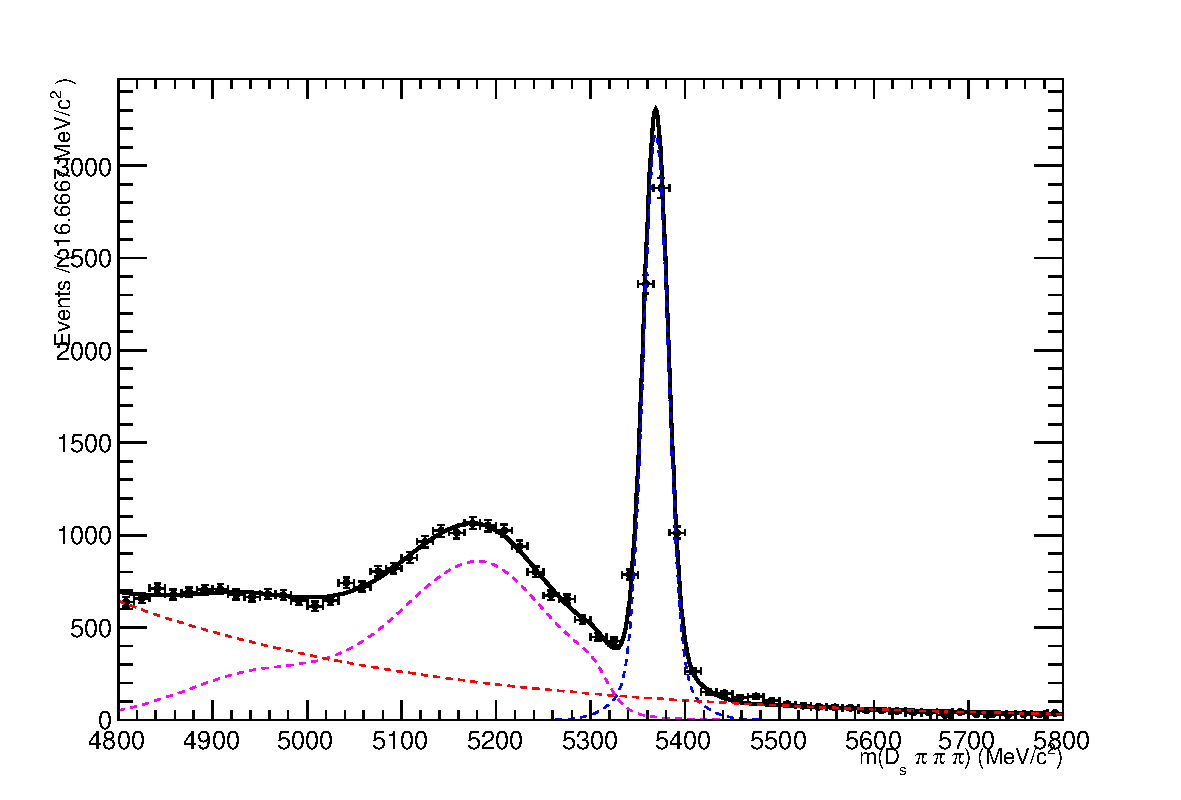
\includegraphics[height=7.cm,width=0.49\textwidth]{figs/3pi_BmassFit_11.pdf}
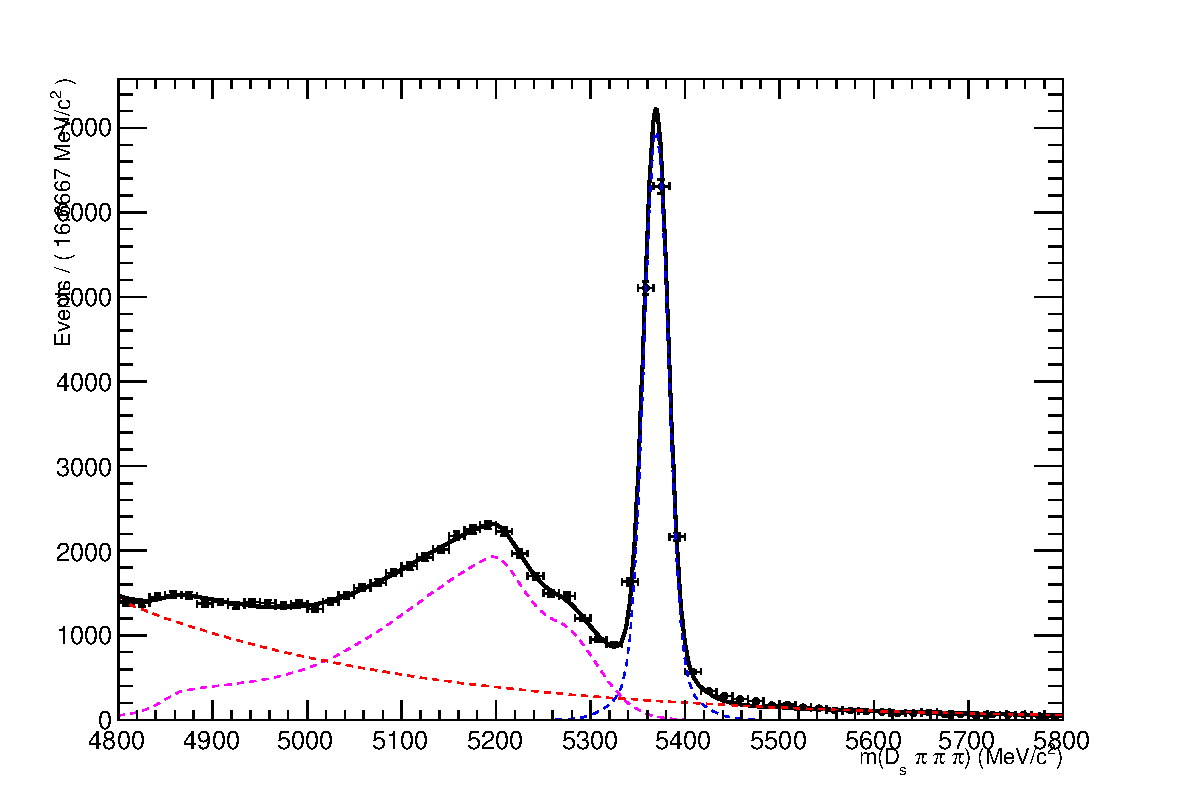
\includegraphics[height=7.cm,width=0.49\textwidth]{figs/3pi_BmassFit_12.pdf}
\caption{Invariant mass distribution of $\Bs\to\Ds\pion\pion\pion$ candidates for (left) 2011 and (right) 2012 data.
A fit described in the text is overlaid. The dashed lines show the (green) partially reconstructed and (red) combinatorial background, as well as the (blue) signal component.}
\label{fig: BsDs3piFit}
\end{figure}

The determined number of $\Bs\to\Ds\kaon\pion\pion$ decays is $6907 \pm 115$ for 2011 data and $14965 \pm 146$ for 2012 data. 
The determined yield for the partially reconstructed $\Bs\to\Ds^{*}\pion\pion\pion$ background is  (2011) $13685 \pm 449$ and (2012)  $28702e+04 \pm 573$, 
while the yield for the combinatorial background is (2011) $12193 \pm 457$ and (2012) $25212 \pm 564$.



\subsection{Fit to $\Bs\to\Ds\kaon\pion\pion$ candidates}
\label{subsec: SigFit}

\begin{figure}[h]
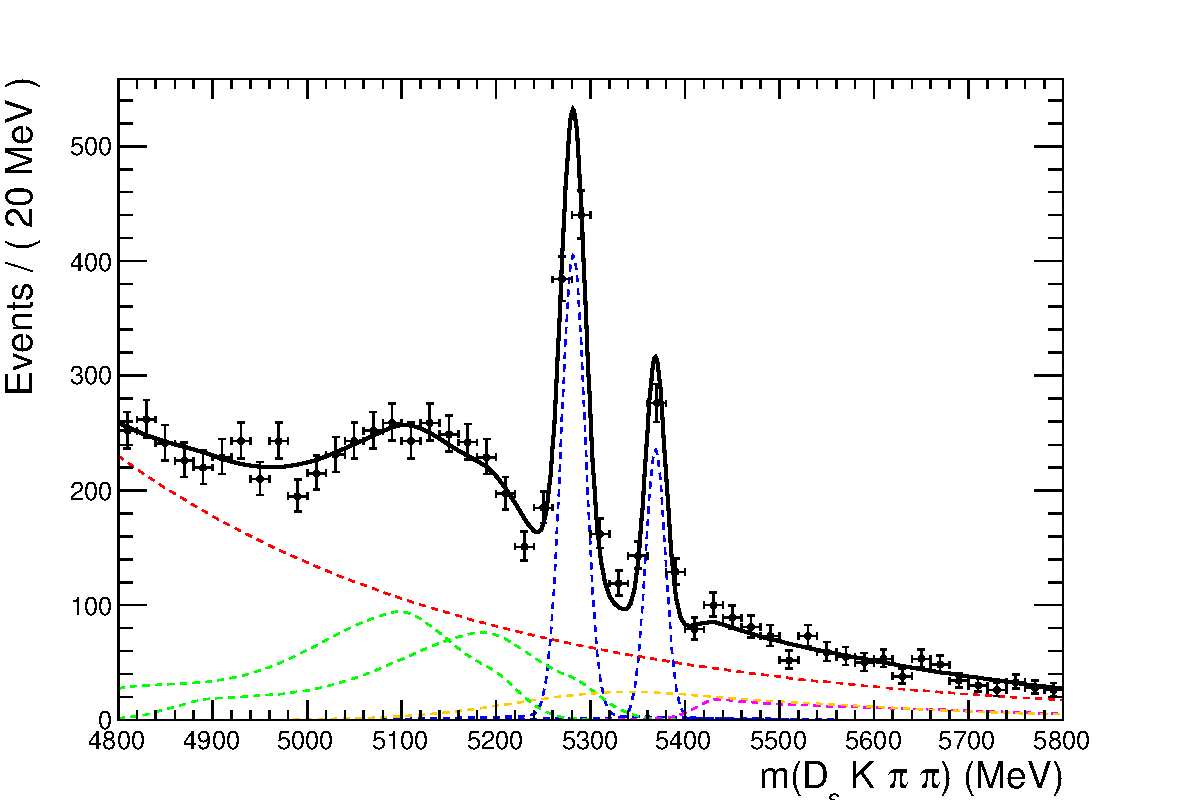
\includegraphics[height=7.cm,width=0.49\textwidth]{figs/BmassFit_11.pdf}
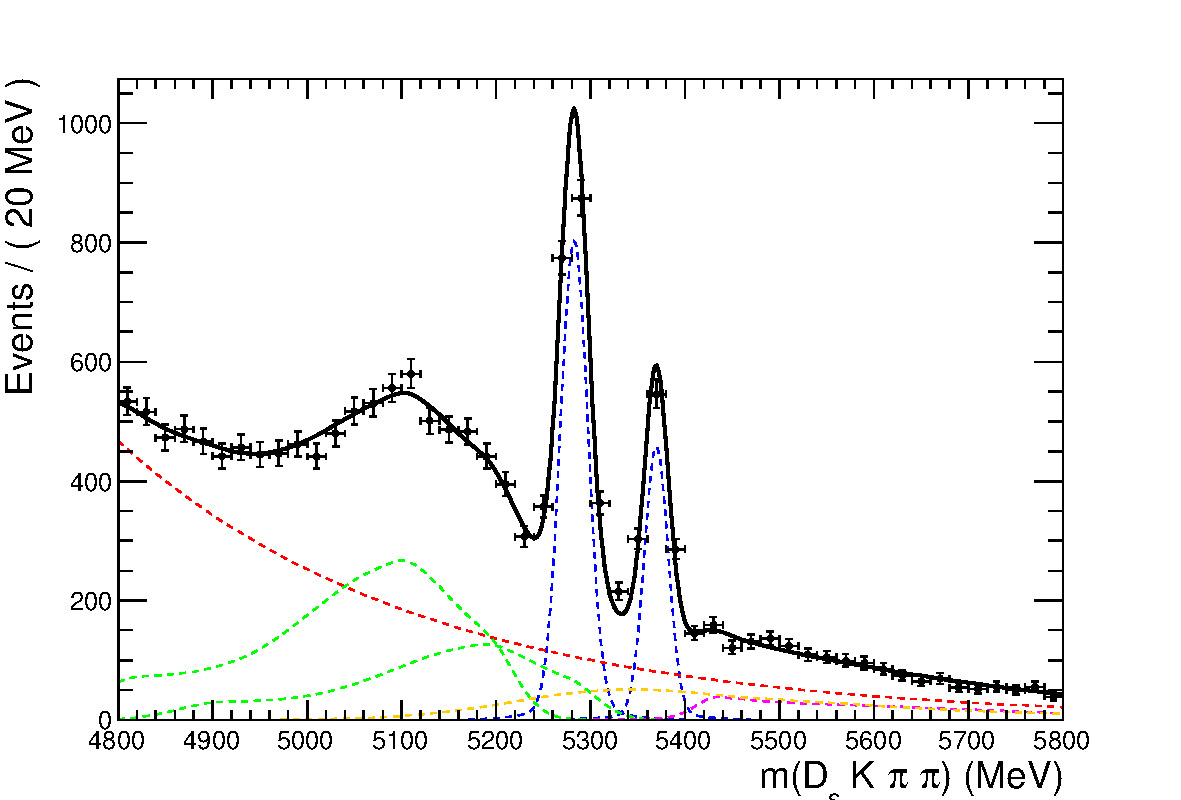
\includegraphics[height=7.cm,width=0.49\textwidth]{figs/BmassFit_12.pdf}
\caption{Invariant mass distribution of $\Bs\to\Ds\kaon\pion\pion$ candidates for (left) 2011 and (right) 2012 data.
A fit described in the text is overlaid. The dashed lines show the (green) partially reconstructed and (red) combinatorial background, as well as the (blue) signal component. 
Additional, the dashed magenta line depicts the miss-ID background and the dashed yellow line shows the miss-identified, partially reconstructed background component.}
\label{fig: BsDsKpipiFit}
\end{figure}


Fig. \ref{fig: BsDsKpipiFit} shows the invariant mass distribution of $\Bs\to\Ds\kaon\pion\pion$ candidates. 
A unbinned maximum likelihood fit is overlaid, which consists of two double gaussian models for the $\Bz$ and $\Bs$ signal, two sums of three bifurcated gaussians for the $\Bs$/$\Bz\to\Ds^{*}\kaon\pion\pion$ partially reconstructed background contributions and two sums of double crystal ball functions for the single miss-ID $\Bs\to\Ds\pion\pion\pion$ and the partially reconstructed, miss-identified $\Bs\to\Ds^{*}\pion\pion\pion$ decays. \newline
The extracted signal yields are (2011) $330 \pm  26$ and (2012) $758 \pm 38$.  


\begin{table}[h]
\centering
\begin{tabular}{l c c}
Decay & yield 2011 & yield 2012\\
\hline
$\Bs\to\Ds\kaon\pion\pion$ &  $330 \pm  26$   &  $758 \pm 38$\\
$\Bs\to\Ds\pion\pion\pion$ &  $6907 \pm 115$  &  $14965 \pm 146$\\
\hline
\end{tabular}
\caption{Summary of signal yields from the fits to 2011 and 2012 data.}
\label{tab: SigYields}
\end{table}

